\documentclass{article}
\usepackage{tikz}
\usetikzlibrary{shapes.geometric, arrows.meta}

\begin{document}

	% stuff goes here

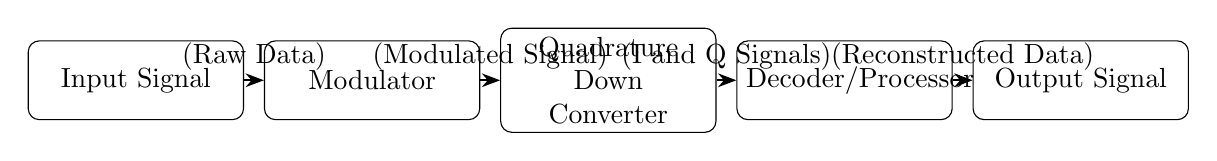
\begin{tikzpicture}[
    % Define block style
    block/.style={rectangle, draw, text width=2.5cm, text centered, rounded corners, minimum height=1cm},
    % Define arrow style
    arrow/.style={-Stealth, thick},
    % Spacing
    node distance=3cm
]

    % Nodes (blocks)
    \node[block] (input) {Input Signal};
    \node[block, right of=input] (modulator) {Modulator};
    \node[block, right of=modulator] (downconverter) {Quadrature Down Converter};
    \node[block, right of=downconverter] (decoder) {Decoder/Processor};
    \node[block, right of=decoder] (output) {Output Signal};

    % Arrows with labels
    \draw[arrow] (input) -- node[above] {(Raw Data)} (modulator);
    \draw[arrow] (modulator) -- node[above] {(Modulated Signal)} (downconverter);
    \draw[arrow] (downconverter) -- node[above] {(I and Q Signals)} (decoder);
    \draw[arrow] (decoder) -- node[above] {(Reconstructed Data)} (output);

\end{tikzpicture}

\end{document}
